\documentclass[uplatex,dvipdfmx]{jsarticle}
\usepackage[top=25truemm,bottom=25truemm,left=25truemm,right=25truemm]{geometry}
\usepackage{graphicx}
\usepackage{color}
\usepackage{amsthm}

\graphicspath{{./images/}}

\newtheorem{thm}{定理}
\newtheorem{dfn}[thm]{定義}
\newtheorem{prob}[thm]{問題}
\newtheorem{lem}[thm]{系}

\begin{document}

\title{最小二乗法とその周辺の数学}
\author{西 航}
\date{2020年1月29日}
\maketitle

この文書は、講座「非専門家のための数学再入門」のための資料です。
当日は基本的には資料がなくても聞けるような話をするつもりですが、
受講して興味を持った人の復習や当日来られなかった人の学習のため、
また時間の都合で省略する部分の補足のために使えるものにするつもりです。

あまりきちんと内容を考えないまま書き始めたのですが、
書き終わってみると、最小二乗法の導入と、
そのガウス分布との関係について説明することをゴールにした文書になったと思います。
ので、この文書のタイトルはそれがわかるようにしました。

各章の内容はおおむね以下のようになっています。
\begin{itemize}
  \item 1章は、ネイピア数 $\mathrm{e}$ の周辺の数学的対象を眺めつつ、
        最終的にはガウス分布という確率分布を紹介するものです。
        積分についても、具体的な計算は省略していますが、説明しています。
  \item 2章は、微分について説明するものです。やはり具体的な計算は省略しています。
  \item 3章は、解を持たない連立方程式の話を導入として最小二乗法を紹介するものです。
        最小二乗法の代表的な適用例である線形回帰についても説明します。
  \item 4章は、尤度という概念と、それに関連する最尤推定という手法を紹介するものです。
        この章の終わりに、最小二乗法とガウス分布の関係について説明します。
\end{itemize}

この文書を読むにあたって、最後に紹介する最小二乗法とガウス分布の関係を理解することを目的にする場合、
1章の内容は少々冗長で、実質的には確率密度関数の節とガウス分布の節だけを読めば十分かもしれません。
一方、2章以降の内容は急ぎすぎで、それぞれの話題について全く知らない場合は
「ちゃんと読まなくても問題ない内容」が少なく、少し辛いかもしれません。

といっても、最小二乗法の周辺の数学を理解したいモチベーションがある人は少ないと思いますので、
とくに何を理解するなどの目的は定めずに、単に「たまには数学的な対象に触れてみたい」とか、
「何でもいいから文章を読みたい」のようなモチベーションで読んでいただければいいと思います。

この文書には正確でない表現や、厳密でない表現が頻繁に使われています。
その点で、これは数学的な文書であると言わんばかりのタイトルをつけるのは
少々心苦しいところですが、ご容赦ください。
もっと厳密な議論について知りたいと思った場合は、
ぜひ書店で入門書を入手して学習を続けていただければと思います。

\tableofcontents

\section{ガウス分布の話}
\subsection{ガウス積分}
  次の数式をご存知でしょうか。
  \begin{equation}
    \label{gaussian-integral}
    \mathrm{e}^{i\pi} = -1
  \end{equation}
  これは、オイラーの等式と呼ばれるものです。
  $\mathrm{e}$ はネイピア数と呼ばれる、 $2.72$ くらいの定数です。
  $i$ は虚数単位で、 $\sqrt{-1}$ のことです。
  $\pi$ は円周率と呼ばれる、 $3.14$ くらいの定数です。
  $\mathrm{e}$, $i$, $\pi$ はそれぞれ、数学のジャンルでいうと、
  解析学、代数学、幾何学で使われるものだと考える人が多いようです。
  数学の中でも違うジャンルで使われる3つの定数がシンプルな等式で関連付けられていることから、
  オイラーの等式は数学において最も美しい等式であると言う人もいるようです。

  では、次の数式はどうでしょうか。
  \[
    \int_{-\infty}^{\infty}\mathrm{e}^{-x^2}dx = \sqrt{\pi}
  \]
  これは、ガウス積分と呼ばれるものです。
  $\mathrm{e}$ と $\pi$ は先程と同じ、ネイピア数と円周率です。
  $\infty$ は、定数ではないのですが、どんな実数よりも大きい状態を表す記号のようなものです。
  $-\infty$ も同様に、どんな実数よりも小さい状態を表す記号のようなものです。
  $\int$ と $dx$ は、積分を表します。積分を知らない人はまだ分からなくてもかまいませんが、
  とにかく、 $\mathrm{e}^{-x^2}$ という関数に積分という操作をすると $\sqrt{\pi}$ になる、ということです。

  筆者には数式の美しさというのはよく分かりませんが、
  オイラーの等式と同じように $\mathrm{e}$ も $\pi$ も登場するし、
  $i$ が出てこない代わりに $\sqrt{~}$ も $\int$ も登場するので、
  美しさは同じくらいじゃないかと思うのですが、どうでしょうか
  \footnote{
    少なくとも世の中では、オイラーの等式を美しいという人に比べて、
    ガウス積分を美しいという人は圧倒的に少ないようです。
  }?

\subsection{$\mathrm{e}$ とは何か}
  まず、 $\mathrm{e}$ について説明します。
  $\mathrm{e}$ の説明には $\log$ と微分を使うので、人によっては、
  知らないものを使って知らないものを説明されることになるかもしれません。
  そういう場合、今のところは
  「よくわからないけどちゃんとした定義があるものなんだ」とか、
  「そういうモチベーションがあるものなんだ」のように、
  気分だけ味わってもらえれば大丈夫です。
  
  次の問題は、 $\log$ (対数)の微分を考えると直面するものです。
  \begin{prob}
    対数関数 $\log_{a}x$ の微分
    \[
      \frac{d}{dx} log_{a}x
    \]
    は何になるか?
  \end{prob}
  これはとても自然な問題です。数学者というのは、関数を見ると微分してみたくなるものなのです
  \footnote{
    これは嘘です。微分してみたくなるかどうかは場合によります。
    ただし、対数関数を微分したくなることは、実用上よくあると思います。
  }。
  証明は省略しますが、この問題は以下の定理によって解決されます。
  \begin{thm}\label{differentiate_log}
    定数 $\mathrm{e}$ が存在して、
    \[
      \frac{d}{dx}\log_{a}x = \frac{1}{x\log_{\mathrm{e}}a}
    \]
    となる。
  \end{thm}
  この定理で登場する $\mathrm{e}$ がネイピア数です。
  細かいことはさておき、対数を扱おうとすると自然に登場する定数であることがわかります。

  さて、定理\ref{differentiate_log}と $\log_{e}{e} = 1$ であることからただちに、次の事実がわかります。
  \begin{lem}
    $\mathrm{e}$ を底とする対数関数の微分は
    \[
      \frac{d}{dx}\log_{\mathrm{e}}x = \frac{1}{x}
    \]
    となる。
  \end{lem}
  このように、 $\mathrm{e}$ を底とする対数のことを、とくに\textbf{自然対数}と呼びます。
  また、 $\mathrm{e}$ のことを\textbf{自然対数の底}と呼ぶこともあります
  \footnote{ネイピア数と自然対数の底は同じものです。}。
  以下、この文書では、特に断らない限り $\log$ の底は $\mathrm{e}$ であるとします。

  指数関数 $a^x$ を考えるときも、 $\mathrm{e}$ はよく登場します。
  \begin{thm}
    指数関数 $a^x$ の微分は
    \[
      \frac{d}{dx}a^x = a^x \log a
    \]
    となる。
  \end{thm}
  対数の場合と同様に、底が $e$ の場合は少しすっきりした見た目になります。
  \begin{lem}
    $\mathrm{e}$ を底とする指数関数の微分は
    \[
      \frac{d}{dx}\mathrm{e}^x = \mathrm{e}^x
    \]
    となる。
  \end{lem}
  つまり、 $\mathrm{e}^x$ は\textbf{微分しても変わらない関数}です。
  一般に、数学者は\textbf{ある操作によって変わらないもの}を見つけるととても嬉しくなります。
  $\mathrm{e}^x$ は、\textbf{関数}という非常に基本的な対象のうち、
  \textbf{微分}という非常に基本的な操作で変わらないものなので、
  これはとても嬉しいことです。

  これも証明は省略しますが、 $\mathrm{e}$ は次のような表示を持ちます:
  \[
    \mathrm{e} = 1 + \frac{1}{1!} + \frac{1}{2!} + \frac{1}{3!} + \cdots
  \]
  ここで、 $n!$ は $n$ の\textbf{階乗}と呼ばれるもので、
  $n! = 1 \times 2 \times 3 \times \cdots \times n$ です。
  指数とか対数を扱うときに $\mathrm{e}$ が現れることの嬉しさは実際に使ってみないとわからないかもしれませんが、
  この表示を見ると「なんかすごそう感」は伝わるのではないでしょうか。

  今後、 $\mathrm{e}$ を底とする指数関数は頻繁に登場します。
  しかも指数部分が複雑な式になることが多いので、 $\exp$ という記号を定義しておきます。
  \begin{dfn}
    $\mathrm{e}$ を底とする指数関数を $\exp(x)$ と書く。
    \[
      \exp(x) := \mathrm{e}^x
    \]
    である。
  \end{dfn}

  この記号を使ってガウス積分を書き直すと、
  \[
    \int_{-\infty}^{\infty}\exp(-x^2)dx = \sqrt{\pi}
  \]
  となります。

\subsection{$\exp(-x^2)$ と積分}
  関数
  \begin{equation}
    \label{gaussian-func}
    y = \exp(-x^2)
  \end{equation}
  のグラフについて考えます。
  グラフの概形については、以下のような観察ができます。
  \begin{itemize}
    \item $x^2$ の関数なので、グラフは原点を中心として左右対称の形になります。
    \item $x = 0$ で最大値 $1$ をとります。
    \item $x$ が原点から離れて大きく、もしくは小さくなるにつれて、グラフの両端は $x$ 軸に漸近しますが、交わったり接することはありません。
  \end{itemize}
  結局、(\ref{gaussian-func})のグラフは図\ref{gaussian1}のようになります。
  \begin{figure}
    \centering
    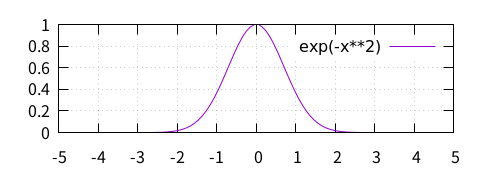
\includegraphics[width=15cm]{gaussian1.png}
    \caption{$y = \exp(-x^2)$ のグラフ}
    \label{gaussian1}
  \end{figure}

  さて、積分というのは、関数のグラフと $x$ 軸で囲まれる部分の面積のことです
  \footnote{
    正確には、グラフが $x$ 軸より下にある部分では積分は負の値になるので、
    符号付き面積とでも呼ぶほうがより正確かもしれません。
  }。
  たとえば $\int_{0}^{1} \exp(-x^2)dx$ であれば、上のグラフと $x$ 軸で囲まれる部分のうち、
  $x = 0$ と $x = 1$ で区切られる部分の面積です。
  ここで、 $[0, 1]$ を積分区間といい、 $0, 1$ をそれぞれ積分区間の下端、上端といいます。

  最初に紹介したガウス積分(\ref{gaussian-integral})は、同じ関数 $\exp(-x^2)$ の積分について、
  上端 $\rightarrow \infty$ と下端 $\rightarrow -\infty$ の極限をとったものです。
  その値は、この文書の冒頭で紹介したとおり、 $\sqrt{\pi}$ となります。

\subsection{関数の平行移動}
  では、関数 $y = \exp(-(x-1)^2)$ のグラフはどうなるでしょうか。
  この関数の $x = 0$における値は、関数(\ref{gaussian-func})の $x = -1$ における値と等しくなります。
  $x = 1$ における値は、(\ref{gaussian-func})の $x = 0$ における値と等しくなります。
  一般に、 $x = a$ における値は、(\ref{gaussian-func})の $x = a - 1$ における値と等しくなります。
  したがって、この関数のグラフは図\ref{gaussian2}のように、
  (\ref{gaussian-func})のグラフを $x$ 軸方向に $1$ だけ平行移動したものになります。
  \begin{figure}
    \centering
    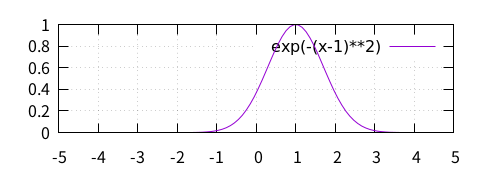
\includegraphics[width=15cm]{gaussian2.png}
    \caption{$y = \exp(-(x-1)^2)$ のグラフ}
    \label{gaussian2}
  \end{figure}
  $x$ 軸方向に平行移動しただけなので、積分の値は変わりません。つまり、
  \[
    \int_{-\infty}^{\infty} \exp(-(x-1)^2) dx = \sqrt{\pi}
  \]
  です。
  もっと一般に、 $x$ 軸方向に $\mu$ だけ平行移動しても積分の値は同じです。つまり、
  \[
    \int_{-\infty}^{\infty} \exp(-(x-\mu)^2) dx = \sqrt{\pi}
  \]
  となります。

\subsection{$x$ 軸方向の拡大/縮小}
  ちょっと違う方向に変形した、 $y = \exp(-(x/2)^2)$ のグラフはどうなるでしょうか。
  $x$ が $x/2$ になっているので、
  この関数の $x = 2$における値は、関数(\ref{gaussian-func})の $x = 1$ における値と等しくなります。
  $x = 4$ における値は、(\ref{gaussian-func})の $x = 2$ における値と等しくなります。
  一般に、 $x = a$ における値は、(\ref{gaussian-func})の $x = a/2$ における値と等しくなります。
  したがって、この関数のグラフは図\ref{gaussian3}のように、
  (\ref{gaussian-func})のグラフを $x$ 軸方向に倍の長さに拡大したものになります。
  \begin{figure}
    \centering
    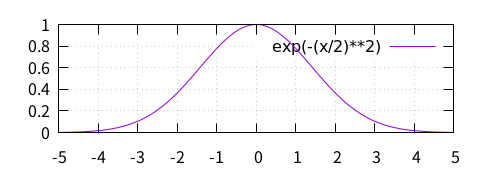
\includegraphics[width=15cm]{gaussian3.png}
    \caption{$y = \exp(-(x/2)^2)$ のグラフ}
    \label{gaussian3}
  \end{figure}
  この場合は、積分の値も変わります。 $x$ 軸方向に倍に伸びているので、面積も倍になります。
  つまり、
  \[
    \int_{-\infty}^{\infty} \exp(-(x/2)^2) dx = 2\sqrt{\pi}
  \]
  です。
  もっと一般に、(\ref{gaussian-func})を $x$ 軸方向に $a$ に拡大すると、面積(積分)も $a$ 倍になります。
  つまり、
  \[
    \int_{-\infty}^{\infty} \exp(-(x/a)^2) dx = a\sqrt{\pi}
  \]
  となります。

\subsection{平行移動と拡大/縮小の組み合わせ}
  平行移動と拡大の両方を組み合わせた、
  \[
    y = \exp(-(\frac{(x-1)}{2})^2)
  \]
  のグラフはどうなるでしょうか。
  この関数の $x = 3$における値は、関数(\ref{gaussian-func})の $x = 1$ における値と等しくなります。
  $x = 5$ における値は、(\ref{gaussian-func})の $x = 2$ における値と等しくなります。
  一般に、 $x = a$ における値は、(\ref{gaussian-func})の $x = (a-1)/2$ における値と等しくなります。
  したがって、この関数のグラフは図\ref{gaussian4}のように、
  (\ref{gaussian-func})のグラフを $x$ 軸方向に倍の長さに拡大してから、
  $1$ だけ平行移動したものになります。
  \begin{figure}
    \centering
    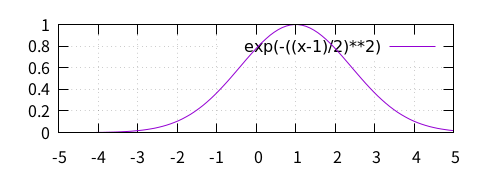
\includegraphics[width=15cm]{gaussian4.png}
    \caption{$y = \exp(-(\frac{(x-1)}{2})^2)$ のグラフ}
    \label{gaussian4}
  \end{figure}
  この場合、積分の値には、拡大した分は効きますが、平行移動の分は関係しません。
  つまり、
  \[
    \int_{-\infty}^{\infty} \exp(-(\frac{(x-1)}{2})^2) dx = 2\sqrt{\pi}
  \]
  です。
  もっと一般に、(\ref{gaussian-func})を $x$ 軸方向に $a$ 倍に引き伸ばしてから $\mu$ だけ平行移動すると、
  面積(積分)は $a$ 倍になります(平行移動の $\mu$ は影響しません)。
  つまり、
  \[
    \int_{-\infty}^{\infty} \exp(-(\frac{(x-\mu)}{a})^2) dx = a\sqrt{\pi}
  \]
  となります。

  また、関数全体を $b$ 倍するとグラフの高さも $b$ 倍になるので、積分の値も $b$ 倍になります。
  つまり、
  \begin{equation}
    \label{gaussian-integral-devided-by-b}
    \int_{-\infty}^{\infty} b \exp(-(\frac{(x-\mu)}{a})^2) dx = ab \sqrt{\pi}
  \end{equation}
  です。

\subsection{確率密度関数}
  ちょっと話がそれるようですが、ここでいったん確率論の話をします。
  確率変数 $X$ は、$0$以上$1$以下の実数値をとるものとします。
  その分布は値の範囲だけからは定まらず、
  \begin{itemize}
  \item とくに出やすさに差のない分布
  \item $0$に近い値ほど出やすい分布
  \item $1$に近い値ほど出やすい分布
  \item 中間の特定の値に近いほど出やすい分布
  \end{itemize}
  など、いろいろ考えられます。
  これらの違いは、図\ref{distributions}のような関数たちによって表現できます。
  \begin{figure}
    \centering
    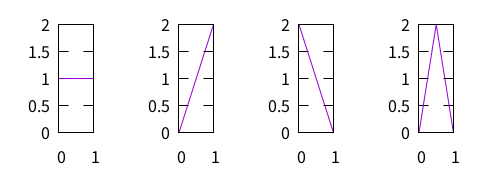
\includegraphics[width=15cm]{distributions.png}
    \caption{確率密度関数たち}
    \label{distributions}
  \end{figure}
  左から、
  出やすさに差のない分布、
  $0$に近い値ほど出やすい分布、
  $1$に近い値ほど出やすい分布、
  $0.5$に近い値ほど出やすい分布
  です。
  確率変数の値がある区間に含まれる確率はこれらの関数の積分で計算されます。
  $0$以上$1/4$以下の区間$[0,1/4]$に含まれる確率を例にすると、
  左から、$1/4, 1/16, 7/16, 1/8$です。
  このように確率変数の分布を表す関数を\textbf{確率密度関数}と呼びます。

  すべての確率密度関数は
  \begin{itemize}
    \item 常に$0$以上の値を取ること
    \item 定義域全体での積分が$1$になっていること
  \end{itemize}
  が必要です。
  この2点が満たされているからこそ、積分によって確率を表現することができます。

\subsection{ガウス分布}
  さて、積分(\ref{gaussian-integral-devided-by-b})で、 $a = \sqrt{2\sigma^2}, b = \frac{1}{\sqrt{2\pi\sigma^2}}$ とすれば、
  \begin{equation}
    \label{integrate-gaussian-distribution}
    \int_{-\infty}^{\infty} \frac{1}{\sqrt{2\pi\sigma^2}} \exp(-\frac{(x-\mu)^2}{2\sigma^2}) dx = 1
  \end{equation}
  となります。
  \begin{figure}
    \centering
    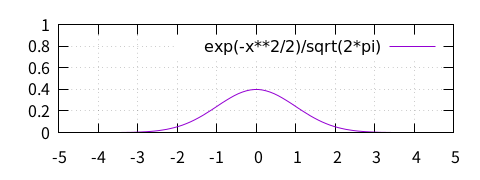
\includegraphics[width=15cm]{gaussian5.png}
    \caption{ガウス分布 $\mu = 0, \sigma = 1$}
    \label{gaussian5}
  \end{figure}
  これは一見、不必要に複雑な式に感じるかもしれませんが、
  $\mu$ と $\sigma$ には確率論的な(統計学的な)意味があるので、こういう表示になっています。
  
  さて、積分が $1$ になるということは、関数
  \begin{equation}
    \label{gaussian-distribution}
    f(x) = \frac{1}{\sqrt{2\pi\sigma^2}} \exp(-\frac{(x-\mu)^2}{2\sigma^2})
  \end{equation}
  は確率密度関数を表していると考えることができます。
  その分布の様子は図\ref{gaussian5}に現れるように
  $\mu$ に近い値ほど多く、それから離れるにつれて少なくなっていくようになります。
  この確率分布を\textbf{ガウス分布}、または\textbf{正規分布}と呼びます。
  
  \begin{dfn}
    ガウス分布について、いくつかの言葉を定義しておきます。
    \begin{itemize}
      \item 関数(\ref{gaussian-distribution})において、
      $\mu$ を分布の\textbf{平均}もしくは\textbf{期待値}、
      $\sigma^2$ を分布の\textbf{分散}と呼びます
      \footnote{
        この2つは確率論や統計学で使われる量で、ガウス分布に限らず、一般に確率分布において重要なパラメータです。
      }。
      \item 平均 $\mu$, 分散 $\sigma^2$ のガウス分布を $N(\mu, \sigma^2)$ で表します。
      \item 平均 $0$, 分散 $1$ のガウス分布 $N(0, 1)$ を特に\textbf{標準正規分布}と呼びます。
    \end{itemize}
  \end{dfn}

  ガウス分布は様々な場面で利用されます。
  例えば科学実験において、測定値には誤差が含まれるため、
  同じ条件で測定を繰り返して真の値を確率論的に推定することがありますが、
  その際、真の値と測定値との誤差はガウス分布に従うと仮定するのが一般的です。

  また、以下のような強力な定理が知られています。
  \begin{thm}[中心極限定理]
    $n$ 個の確率変数 $X_1, \cdots, X_n$ は独立で、同じ確率分布に従い、
    期待値 $\mu$, 分散 $\sigma^2$ を持つとする。
    このとき、確率変数
    \[
      Y_n = \frac{\sqrt{n}(\frac{X_1 + \cdots + X_n}{n} - \mu)}{\sigma}
    \]
    は標準正規分布に分布収束する。
  \end{thm}
  \textbf{独立}とか\textbf{分布収束}の意味はわからなくても構いません。
  少し誇張した表現をすると、この定理の言っていることは、
  「確率変数がもともとどんな分布に従うとしても
  \footnote{ここが誇張です。正確には、分布の分散が有限である必要があります。}、
  値をたくさんとって平均すると、ガウス分布に従う」
  ということです。
  これは非常に強力な定理です。この定理があるからこそ、ガウス分布は非常に重要な確率分布です。


\section{微分の話}
\subsection{微分ってなに?}
  微分について何も知らないという人はそれほど多くないと思います。
  ほとんどの人は、何らかの微分は計算した経験があるのではないでしょうか
  \footnote{って書けてしまう社会けっこうすごい}。
  この章では、関数
  \begin{equation}
    f(x) = x^3 - 3x
  \end{equation}
  について調べながら、微分ができると何ができるのか、何が嬉しいのかを説明します。

  では、微分とは何でしょうか。
  微分とは、誤解を恐れずに断言すれば、接線の傾きです。

  \begin{figure}
    \centering
    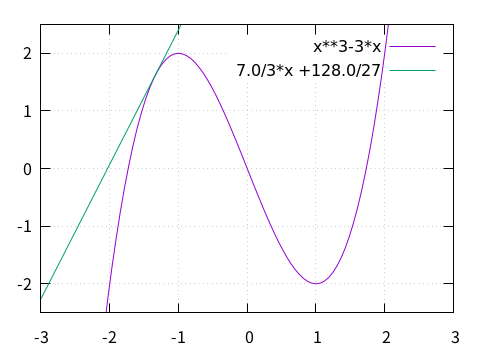
\includegraphics[width=8cm]{diff1.png}
    \caption{$y = x^3 -3x$ のグラフとその接線}
    \label{diff1}
  \end{figure}

  正確には、接線の傾きは微分係数と呼ばれます。
  図\ref{diff1}のように、 $y = f(x)$ 上の点 $(-4/3, 44/27)$ における接線は
  \[
    y = 7/3x +128/27
  \]
  です。
  つまり接線の傾きは $7/3$ なので、 $f(x)$ の $x = -4/3$ における微分係数は
  \[
    f'(-4/3) = 7/3
  \]
  です。
  接線の傾きはもちろん $x$ の値によって変わります。つまり、 $x$ の関数です。
  このように、もとの関数に対して、その各点における接線の傾きを考えることで
  別の関数を作ることができます。
  その関数がもとの関数の微分と呼ばれるものです。
  記号としては、 $f'(x)$ や $\frac{d}{dx}f(x)$ などが使われます。
  具体的な計算の過程は省略しますが、$f(x) = x^3 -3x$ の場合、微分は
  \[
    f'(x) = 3x^2 -3
  \]
  となります。

\subsection{微分ができると近似ができる}
  微分を使うと、関数の近似ができます。
  つまり、局所的な情報から大域的な情報を推定することができます。
  ここでは、 $f(x) = x^3 -3x$ の $x = -4/3$ 付近における様子から、
  $f(x)$ の全体的な様子を推定する問題を考えます。

  微分を知らなくても理解できる、もっとも素朴な近似は、わかっている値をそのまま使うものです。
  $f(-4/3) = 44/27$ なので、 $x$ の値によらず
  \[
    f(x) \simeq \frac{44}{27}
  \]
  という近似です\footnote{$\simeq$ は、左辺が右辺によって近似される、の意味で使っています。}。

  次に考えられる、もう少し高度な近似は、微分を1回使うものです。
  先ほど解説したように、$f(-4/3) = 44/27, f'(-4/3) = 7/3$ なので、
  $y = f(x)$ の点 $(-4/3, 44/27)$ における接線の傾きは $7/3$ です。
  つまり、この接線は $y - 44/27 = 7/3(x + 4/3)$ で表されます。
  接線は関数の近似であると考えると、これを整理して
  \[
    f(x) \simeq \frac{7}{3}x + \frac{128}{27}
  \]
  と近似することができます。
  図\ref{diff1}は、この近似の様子をグラフで表したものです。
  少なくとも $x = -4/3$ 付近では、微分を使わない $f(x) \simeq 44/27$ よりは
  まともな近似になっていることが見て取れると思います。

  さらに微分を何度も使うことで、もっと近似の精度を上げることができます。
  次の定理は解析学において非常に基礎的で重要な定理です。

  \begin{thm}[Taylorの定理]
    $f(x)$ が実数全体で $n$ 回微分可能であるとき、
    \[
      f(x) = f(a) + \frac{f'(a)}{1!}(x-a) + \frac{f''(a)}{2!}(x-a)^2 + \cdots + \frac{f^{(n-1)}(a)}{(n-1)!}(x-a)^{n-1} + \frac{f^{(n)}(\theta(x-a))}{n!}(x-a)^n
    \]
    を満たす $\theta$ ($0 < \theta < 1$) が存在する。

    ただし、$f''$は$f$を$2$回微分したもの、$f^{(n)}$は$f$を$n$回微分したもの。
    $n!$ は $n$ の階乗。
  \end{thm}

  Taylorの定理は、ひとことで言えば、関数を多項式で近似する定理です。
  最後の項だけ他と少し様子が違うのは、誤差を吸収するためです。
  $n$ が大きくなると分母の $n!$ は爆発的に大きくなるため、
  項を増やす(つまり、微分の回数を増やす)につれて誤差は小さくなります
  \footnote{これは厳密には嘘です。もとの関数によります。}。

  \begin{figure}
    \centering
    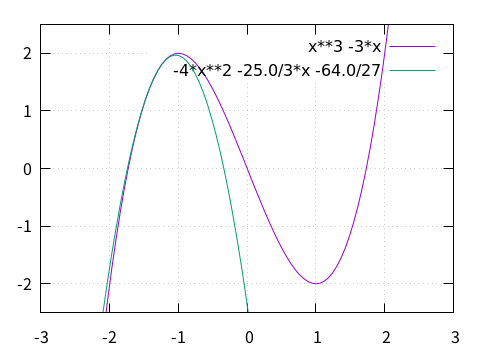
\includegraphics[width=8cm]{diff2.png}
    \caption{$y = f(x)$ のグラフとその2次近似}
    \label{diff2}
  \end{figure}

  図\ref{diff2}は、 $f(x)$ をTaylorの定理によって $x=a$ を中心に多項式に展開し、
  2次の項までで打ち切った
  \[
    f(x) \simeq -4x^2 -\frac{25}{3}x -\frac{64}{27}
  \]
  のグラフです。
  $x = -4/3$ 付近では、
  $f(x) \simeq \frac{44}{27}$ や
  $f(x) \simeq \frac{7}{3}x + \frac{128}{27}$ よりもよい近似になっていることが見て取れると思います
  \footnote{3次の項までを使うと、もとの関数と完全に一致します。もともと3次式であるためです。}。

\subsection{微分ができると極値がわかる}
  微分を使う目的で最も多いのは、おそらく、\textbf{極値}を見つけるためだと思います
  \footnote{本当かどうかは知りませんが、たぶん。}。
  極値とは、極大値と極小値をまとめて呼ぶ言い方で、
  ある点の近傍での最大値や最小値のことです。
  やはり $f(x) = x^3 -3x$ を例に取ると、グラフを見て推測できるように、
  この関数は $x = -1$ で極大値 $2$ を、 $x = 1$ で極小値 $-2$ をとります。

  関数の極値では、微分が $0$ になる
  \footnote{言い換えれば、極値では接線の傾きが0になるということです。これは納得しやすいと思います。}
  ことが知られています。
  逆に言えば、微分が $0$ になる点は極値の候補なので、極値を効率的に探すことができます。
  $f(x) = x^3 -3x$ であれば、
  \[
    f'(x) = 3x^2 - 3
  \]
  で、 $f'(x) = 0$ ならば $x = \pm 1$ です。
  したがって、 $f(x)$ が極値をとるような $x$ の値の候補は $x = \pm 1$ のみです。
  きちんと調べると、$f$ は $x = 1$ でも $x = -1$ でも極値をとることがわかります。

\section{最小二乗法の話}
\subsection{連立方程式を解く}
  連立方程式を1つも解いたことがない人は、おそらくほとんどいないと思います
  \footnote{それもけっこうすごいことだと思う。}。
  連立方程式とは、例えば以下のようなものです。

  \begin{equation}
    \left\{
    \begin{array}{lll}
      x + y - 3 &=& 0 \\
      3x - y - 1 &=& 0
    \end{array}
    \right.
  \end{equation}

  これは多くの人が解けるのではないでしょうか。
  2つの方程式を足して $4x - 4 = 0$ が分かってしまえばあとは簡単で、
  $x = 1, y = 2$ が解となります。

  \begin{figure}
    \centering
    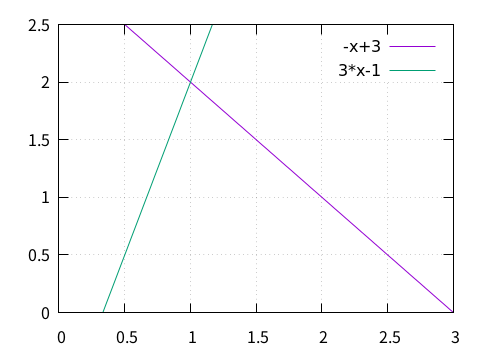
\includegraphics[width=8cm]{simul1.png}
    \caption{$x + y - 3 = 0, 3x - y - 1 = 0$}
    \label{simul1}
  \end{figure}

  図\ref{simul1}はこの状況を表すものです。
  $x + y - 3 = 0$ は右に行くにつれて下がっていく直線、
  $3x - y - 1 = 0$ は右に行くにつれて上がっていく直線で、
  2つの直線の交点 $(1, 2)$ が連立方程式の解となっています。

\subsection{解のない連立方程式を解く}
  では、次の連立方程式は解けるでしょうか。

  \begin{equation}
    \label{unresolvable-simul-eq}
    \left\{
    \begin{array}{lll}
      x + y - 3 &=& 0 \\
      3x - y - 1 &=& 0 \\
      x - 3y + 1 &=& 0
    \end{array}
    \right.
  \end{equation}
  
  1つめと2つめの方程式を連立して解くと、 $x=1, y=2$ となります。
  1つめと3つめの方程式を連立して解くと、 $x=2, y=1$ となります。
  したがって、この連立方程式は解を持ちません。
  つまり、この3つの方程式を同時に満たす実数の組 $(x, y)$ は存在しません。

  \begin{figure}
    \centering
    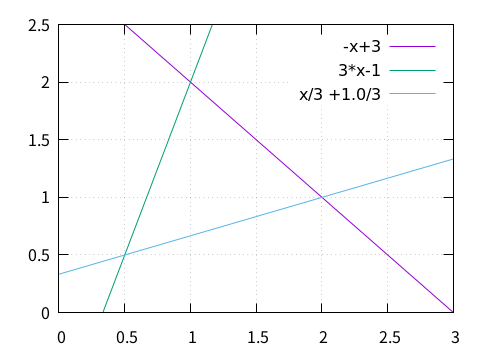
\includegraphics[width=8cm]{simul2.png}
    \caption{$x + y - 3 = 0, 3x - y - 1 = 0, x - 3y + 1 = 0$}
    \label{simul2}
  \end{figure}

  図\ref{simul2}はこの状況を表すものです。
  3つの直線がたまたま1点で交わったり、
  3つの直線のうち2つがたまたま重なっていたりしない限り、
  このような連立方程式は解を持たないことが見て取れます。
  一般に、未知数の個数よりも式の個数が多い連立方程式は、ふつう解を持ちません。

  しかし実用上、測定値に誤差が含まれるような実験を行う場合などで、
  このような連立方程式を解く必要がある状況が存在します
  \footnote{
    勢いで断言しましたが、実際にそういう状況があるかどうかは、実は筆者は知りません。
    光学の研究分野では実際にあるらしいという噂を聞いたことはあります。
  }。
  正確な表現をすれば、\textbf{解}はあくまで存在しないので、「解く」とは言えないかもしれません。
  どの方程式も\textbf{できるだけ満たす}ような、いわば「落とし所を探る」という表現が適切かもしれません。

  方程式を\textbf{できるだけ満たす}というのは、素朴に考えるとあまり意味のない表現です。
  上に挙げたような方程式でいえば、実数の組 $(x,y)$ は方程式を正確に満たすか、そうでないかのどちらかしかありません。
  しかし図形的に考えると、点 $(x_0,y_0)$ が直線 $ax +by +c = 0$ から離れるに従って、
  $ax_0 +by_0 +c$ の値は $0$ から離れていきます
  \footnote{
    点$(x_0,y_0)$が直線$ax+by+c=0$の上にあるときにこの値が0になることを考えると納得しやすいと思います。
  }。
  そこで、以下の関数を考えます。
  \begin{equation}
    \label{square-sum-of-simul-eq}
    f(x,y) = (x+y-3)^2 + (3x-y-1)^2 + (x-3y+1)^2
  \end{equation}
  これは、連立方程式(\ref{unresolvable-simul-eq})の左辺をそれぞれ2乗して足したものです。
  各項は(2乗されているので)$0$以上の値をとり、
  点 $(x,y)$ がそれぞれの直線に近ければ近いほど小さくなります。
  $f(x,y)$ はそれらの和なので、 $f(x,y)$ が小さいほど、
  点 $(x,y)$ は直線たちにバランス良く近い位置にあると考えることができます。
  したがって、 $f(x,y)$ を最小化する問題を考えます。
  
  \begin{prob}
    関数
    \[
      f(x,y) = (x+y-3)^2 + (3x-y-1)^2 + (x-3y+1)^2
    \]
    が最小になるような $x,y$ の値はそれぞれいくつでしょうか。
  \end{prob}

  この問題は微分を使って解決できます。
  $f$ を $x$ で偏微分\footnote{
    偏微分という用語は説明していませんが、ただの微分だと思って問題ありません。
  }した $f_x$ と $y$ で偏微分した $f_y$ はそれぞれ
  \[
    \left\{
    \begin{array}{lll}
      f_x(x,y) &=& 22x -10y -10 \\
      f_y(x,y) &=& -10x +22y -10
    \end{array}
    \right.
  \]
  となります。
  微分の話の章で説明したように、 $f(x,y)$ が最小になるような $(x,y)$ では、
  この微分は $0$ になる必要があります。
  したがって、連立方程式
  \[
    \left\{
    \begin{array}{lll}
      22x -10y -10 &=& 0 \\
      -10x +22y -10 &=& 0
    \end{array}
    \right.
  \]
  を解いて、極値の候補 $(x,y) = (5/6, 5/6)$ が得られます。
  きちんと調べると、これは関数 $f(x,y)$ の最小値を与える $(x,y)$ であることがわかります。

  以上のことから、連立方程式(\ref{unresolvable-simul-eq})の\textbf{落とし所}として
  $(x,y) = (5/6, 5/6)$ が得られることがわかりました。
  実際、3つの方程式の左辺にそれぞれ代入してみると
  \[
    \left\{
    \begin{array}{lll}
      x + y - 3 &=& -4/3 \\
      3x - y - 1 &=& 2/3 \\
      x - 3y + 1 &=& -2/3
    \end{array}
    \right.
  \]
  となり、それなりに $0$ に近い値になります。

  上記の解法で最小化した関数(\ref{square-sum-of-simul-eq})の各項は、
  素朴な観察から分かった「直線から離れるにつれて大きくなる量」(の2乗)でした。
  離れるにつれて大きくなる量といえば、\textbf{距離}が思いつきます。
  点と直線の距離については、以下の定理が知られています。

  \begin{thm}
    方程式 $ax +by +c = 0$ で表される直線と点 $(x_0, y_0)$ との距離は、
    \[
      \frac{|ax_0 +by_0 +c|}{\sqrt{a^2 +b^2}}
    \]
    である。( $|\cdot|$ は絶対値)
  \end{thm}

  このことを使って、次の関数を最小化することを考えてもいいかもしれません:
  \[
    g(x,y) = \frac{(x+y-3)^2}{2} + \frac{(3x-y-1)^2}{10} + \frac{(x-3y+1)^2}{10}
  \]
  つまり、各直線からの距離の二乗和が最小になるような点を探すということです。
  計算は省略しますが\footnote{といっても、 $f$ の場合と同様に、微分を使うだけです。}、
  この関数を最小化する $(x,y)$ を計算すると $(x,y) = (17/14, 17/14)$ となり、
  この点とそれぞれの直線との距離は
  \[
    \left\{
    \begin{array}{lllll}
      |x + y  - 3| /\sqrt{2}  &=& 2\sqrt{2}/7 &=& 0.404\cdots \\
      |3x - y - 1| /\sqrt{10} &=& \sqrt{10}/7 &=& 0.451\cdots\\
      |x - 3y + 1| /\sqrt{10} &=& \sqrt{10}/7 &=& 0.451\cdots
    \end{array}
    \right.
  \]
  となります。

  では、 $(x,y) = (5/6, 5/6)$ と $(x,y) = (17/14, 17/14)$ のどちらがより\textbf{よい解}でしょうか。
  それは、わかりません。
  場合による、という表現のほうが正確かもしれません。
  そもそもこの連立方程式は解を持たないもので、これらは解というよりは、
  それぞれの方程式にバランス良く配慮した落とし所とでも呼ぶべきものでした。
  このように本来解きようがない問題を
  \textbf{不良設定問題} (ill-posed problem, ill-conditioned problem)
  と言います。
  特に、今回紹介したように変数に比べて制約が多すぎる(制約同士が矛盾している)ような問題は
  \textbf{優決定} (overdetermined) であると表現されます。
  逆に、制約が足りずに解が定まらないような問題もあり、
  そのような問題は\textbf{劣決定} (underdetermined) であると表現されます。

  \textbf{機械学習}という言葉は最近バズワードとなっていますが、
  機械学習による解決が話題になるような
  \begin{itemize}
    \item 有名人の顔が写った写真から、その人の名前を判断する
    \item 日本語の文章を英訳する
  \end{itemize}
  などの問題は、本質的に不良設定です
  \footnote{
    有名人によく似た人はけっこういるし、
    文脈によって意味の変わる文章はたくさんあります。
  }。
  それまでに学習した知識から、正しいと思われるものを推定するしかないのです。
  そのような不良設定問題を解決するためにしばしば使われる手法が、
  先ほど解を持たない連立方程式を無理やり解いたときのように、
  \textbf{二乗和を最小化する}というものです
  \footnote{
    すべての機械学習が二乗和を最小化するものだというわけではありません。念のため。
  }。

\subsection{線形回帰}
  二乗和を最小化することで解決できる不良設定問題の例として、\textbf{線形回帰}の問題を紹介します。
  \begin{prob}
    \label{prob:linear-regression}
    次のデータは、日本の5歳から17歳までの男性の、年齢ごとの身長(cm)と体重(kg)の平均値です。
    (https://www.e-stat.go.jp/dbview?sid=0003146500 より)

    \begin{table}[htb]
      \begin{tabular}{lllllllllllll}
        110.3 & 116.5 & 122.5 & 128.1 & 133.7 & 138.8 & 145.2 & 152.7 & 159.8 & 165.3 & 168.4 & 169.9 & 170.6 \\
        18.9 & 21.4 & 24.1 & 27.2 & 30.7 & 34.1 & 38.4 & 44.0 & 48.8 & 54.0 & 58.6 & 60.6 & 62.4
      \end{tabular}
    \end{table}

    \begin{figure}
      \centering
      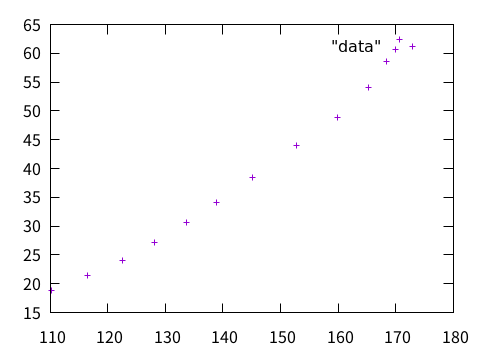
\includegraphics[width=8cm]{scatter1.png}
      \caption{身長と体重の散布図}
      \label{scatter1}
    \end{figure}

    ただし、年齢は無視しています。
    図\ref{scatter1}は、これをプロットしたものです。
    やや乱暴ですが、年齢には関係なく、単に13人分のデータだと思ってください。
    では、身長が150cmの人の体重は平均的にはどのくらいだと考えられるでしょうか。
  \end{prob}

  この問題を解くアプローチとして、身長と体重の間に
  \begin{equation}
    \label{linear-correspondence}
    \mbox{体重} = a \times \mbox{身長} + b
  \end{equation}
  というシンプルな関係を仮定することにします
  \footnote{それが妥当かどうかはいったん考えないことにします。}。
  このパラメータ $a, b$ を決定できれば、身長が150cmの人の体重を推定することができます。

  さて、最初の3人の身長と体重をこの式に当てはめてみると、
  \[
    \left\{
    \begin{array}{lll}
      18.9 &=& 110.3a +b \\
      21.4 &=& 116.5a +b \\
      24.1 &=& 122.5a +b
    \end{array}
    \right.
  \]
  となります。
  1つめと2つめの方程式を連立して解くと $(a,b) = (0.403\cdots, -27.575\cdots)$ 、
  1つめと3つめの方程式を連立して解くと $(a,b) = (0.426\cdots, -28.113\cdots)$ となり、解がありません。
  最初の3人を考えるだけでも、(\ref{linear-correspondence})のような関係は成り立たないということです。
  ともあれ、先ほどと同じように、誤差の二乗和を最小化することを考えます。
  \[
    f(a,b) = (110.3a+b-18.9)^2 + (116.5a+b-21.4)^2 + \cdots + (170.6a+b-62.4)^2
  \]
  数字が大きいので計算の過程は省略しますが、やはり先ほどと同じ方法で
  $(a,b) = (0.719\cdots, -63.838\cdots)$ で最小となることがわかります。
  $150.0 \times 0.719 -63.838 = 44.0\cdots$ なので、
  身長が150cmの人の体重は44kg程度と推定することができます。

  \begin{figure}
    \centering
    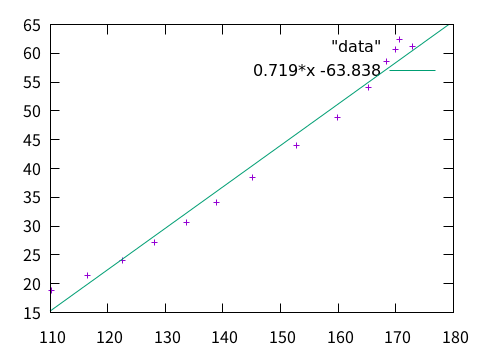
\includegraphics[width=8cm]{scatter2.png}
    \caption{身長と体重の散布図とその回帰直線}
    \label{scatter2}
  \end{figure}

  この推定を信用すれば、一般に、身長と体重の間には
  \[
    \mbox{体重} = 0.719 \times \mbox{身長} - 63.838
  \]
  という関係があることを期待できます。
  図\ref{scatter2}は、その直線を散布図に重ねたものです。
  このように、(誤差を含む)2つの変数
  \footnote{
    一方の変数が原因、もう一方の変数がその結果という関係にあることを期待します。
  }
  の関係を明らかにする手法を\textbf{回帰分析}といいます。
  特に、今回のように直線を当てはめることで関係を調べる場合を\textbf{線形回帰}といい、
  その直線のことを\textbf{回帰直線}といいます。

  この章で何度か使ったテクニックとして、何らかのパラメータを決定する際、
  \textbf{誤差の二乗和を最小化}するものを選ぶというものがありました。
  これを\textbf{最小二乗法}と言います。

\section{最尤推定の話}
\subsection{尤度と最尤法}
  以下の問題を考えます。

  \begin{prob}
    \label{prob:likelihood}
    値 $0$ をとる確率が $p$ , 値 $1$ をとる確率が $1-p$ の確率分布を考えます。
    ここから標本として $0, 0, 0, 0, 1$ の $5$ つの値が得られたとします。
    このとき、 $p$ はいくつであると考えるのが合理的でしょうか。
  \end{prob}
  
  $p$ がいくつであっても( $0$ や $1$ は例外ですが)標本 $0, 0, 0, 0, 1$ が得られる可能性はあるので、
  これは不良設定問題です。
  しかし、これだけの情報から $p$ の「それらしい」値を推定することはできます。
  その状況証拠として、次の問題を考えてみてください。

  \begin{prob}
    問題\ref{prob:likelihood}の状況で、
    \begin{itemize}
      \item $p = 0.4$ であるという説(つまり、 $0$ のほうが $1$ よりもやや出にくいという説)と、
      \item $p = 0.5$ であるという説(つまり、 $0$ も $1$ も等確率で得られるという説)と、
      \item $p = 0.6$ であるという説(つまり、 $0$ のほうが $1$ よりもやや出やすいという説)では、
    \end{itemize}
    どれがより「もっともらしい」でしょうか?
  \end{prob}
  
  標本は $5$ つ中 $4$ つが $0$, $1$ つだけが $1$ なので、
  この中だと、 $p = 0.6$ が一番もっともらしいように思われます。

  問題\ref{prob:likelihood}のような標本が得られる確率を $L(p)$ と書くことにすると
  $L(p) = p^4(1-p)$ なので、
  \[
    L(0.4) = 0.0256, L(0.5) = 0.03125, L(0.6) = 0.05184
  \]
  です。
  したがって、やはり $p = 0.4, 0.5, 0.6$ の中では、 $0.6$ が一番もっともらしいと思われます。
  この判断では、暗黙のうちに「標本は確率最大のものが実現した結果である」ことを仮定しています。
  この仮定を\textbf{最尤原理}\footnote{「さいゆうげんり」と読みます。}と呼びます。

  では、問題\ref{prob:likelihood}を最もよく解決する $p$ は、具体的にいくつでしょうか。
  これはつまり、 $L(p)$ を最大にする $p$ を計算すればよいことになります。
  $L(p)$ の微分を計算して整理すると $dL(p)/dp = p^3(4-5p)$ となり、
  これが $0$ になるのは $p = 0, 4/5$ のときです。
  きちんと調べると、 $L(p)$ は $p = 4/5 = 0.8$ で最大値をとることがわかります。

  問題\ref{prob:likelihood}に関するここまでの議論を整理すると、
  \begin{itemize}
    \item $p = 0.4, 0.5, 0.6$ の中だと、 $p = 0.6$ が一番それらしい。
    \item それは、標本 $0, 0, 0, 0, 1$ が得られる確率を
      $p = 0.4, 0.5, 0.6$ それぞれの場合について計算すると $0.6$ の場合が最大になるからである。
    \item もっと正確に、確率を $p$ の関数として表現した $L(p)$ を
      最大化する $p$ の値を計算すると $p = 0.8$ となった。
    \item したがって、問題\ref{prob:likelihood}の $p$ は $0.8$ であると考えるのが合理的である。
  \end{itemize}
  ということになります。
  $L(p)$ はもっともらしさを表す関数とみなすことができます。
  そのもっともらしさを\textbf{尤度}、尤度を表す関数を\textbf{尤度関数}と呼びます。

  このように、
  \begin{itemize}
    \item 得られた標本からもとの分布のパラメータを決定する問題において
    \item 最尤原理(標本は確率最大のものが実現した結果であるという仮定)に基づいて
    \item 尤度関数を最大化するようなパラメータを選択する
  \end{itemize}
  ような手法を\textbf{最尤推定}または\textbf{最尤法}
  \footnote{
    「尤」は「もっともらしい」(尤もらしい)の尤で、
    「最も尤もらしい」パラメータを求めるという意味です。
  }と呼びます。

\subsection{ガウス分布と尤度と最小二乗の話}
  さて、問題\ref{prob:linear-regression}について改めて考えてみます。
  13人の身長と体重の対応は、以下のようなものでした。
  \begin{table}[htb]
    \begin{tabular}{lllllllllllll}
      110.3 & 116.5 & 122.5 & 128.1 & 133.7 & 138.8 & 145.2 & 152.7 & 159.8 & 165.3 & 168.4 & 169.9 & 170.6 \\
      18.9 & 21.4 & 24.1 & 27.2 & 30.7 & 34.1 & 38.4 & 44.0 & 48.8 & 54.0 & 58.6 & 60.6 & 62.4
    \end{tabular}
  \end{table}

  この問題は最尤法を使っても解決することができます。
  ただし、
  \begin{equation}
    \label{linear-correspondence-with-errors}
    \mbox{体重} = a \times \mbox{身長} + b + \mbox{ガウス分布に従う誤差}e_i
  \end{equation}
  という関係を仮定します。(関係\ref{linear-correspondence}と見比べてみてください。)
  すなわち、
  \[
    e_i = \mbox{体重} - a \times \mbox{身長} -b
  \]
  がガウス分布に従うということです。
  ただし、誤差なので、そのガウス分布の平均は $\mu = 0$ と仮定します。
  また、分散は身長や体重によらず一定で、 $\sigma_0^2$ とします。

  この仮定のもとで、最尤推定によって $a, b$ を推定します。
  ガウス分布の確率密度関数は一般には
  \[
    \frac{1}{\sqrt{2\pi\sigma^2}} \exp(-\frac{(x-\mu)^2}{2\sigma^2})
  \]
  でした。
  $e_i$ が平均 $0$ ,分散 $\sigma_0^2$ のガウス分布に従うことから、
  標本 $e_i$ に対する尤度は
  \[
    \frac{1}{\sqrt{2\pi\sigma_0^2}} \exp(-\frac{e_1^2}{2\sigma_0^2})
    \times
    \frac{1}{\sqrt{2\pi\sigma_0^2}} \exp(-\frac{e_2^2}{2\sigma_0^2})
    \times \cdots \times
    \frac{1}{\sqrt{2\pi\sigma_0^2}} \exp(-\frac{e_{13}^2}{2\sigma_0^2})
  \]
  となり
  \footnote{
    厳密には、確率密度関数の各点における値は確率を表さないので(確率を表すのは積分)、
    さきほど説明した尤度とは少し性質の違うものですが、これも尤度です。
    この違いは、確率分布が離散的か連続的かの違いに由来するものです。
  }、これを整理して $e_i = \mbox{体重} - a \times \mbox{身長} -b$ を代入すると
  尤度関数
  \[
    L(a,b) = \frac{1}{(\sqrt{2\pi\sigma_0^2})^{13}} \exp(-\frac{(18.9-110.3 \times a -b)^2+\cdots+(62.4-170.6 \times a -b)^2}{2\sigma_0^2})
  \]
  が得られます。
  $L(a,b)$ を最大化する $(a, b)$ について調べましょう。

  係数 $1/(\sqrt{2\pi\sigma_0^2})^{13}$ は $a, b$ によらない正の定数です。
  $\exp$ は、中身が大きければ大きいほど全体として大きくなるので、 $\exp$ の中身を最大化すればOKです。
  $\exp$ の中身は全体にマイナスの符号がついており、分母は正なので結局、分子の
  \[
    (18.9-110.3 \times a -b)^2+\cdots+(62.4-170.6 \times a -b)^2
  \]
  を最小化すればよいことになります。
  これは、最小二乗法によるアプローチと同じです。

  すなわち、2つの変数について、一方の変数がもう一方の変数を説明する様子を解析する際、
  \begin{itemize}
    \item 最小二乗法によってパラメータを決定する方法と
    \item 誤差がガウス分布に従うと仮定して最尤推定を行う方法は
  \end{itemize}
  全く同じことであると言えます。
  この事実が、最小4乗法でも最小6乗法でもなく最小2乗法を採用する理由になっています
  \footnote{
    4乗や6乗も、それはそれで何らかの理由付けができるかもしれませんが、
    誤差がガウス分布に従うという仮定はかなり自然なものです。
    それから、身も蓋もないことを言えば、4乗や6乗よりも2乗のほうが計算が簡単です。
  }。

\begin{thebibliography}{9}
  \bibitem{diff} 上見練太郎ほか, 『微分』, 共立出版株式会社, 1995, (ISBN 4-320-01485-5)
  \bibitem{stat} 東京大学教養学部統計学教室編, 『統計学入門』, 東京大学出版会, 1991, (ISBN 978-4-13-042065-5)
\end{thebibliography}

\end{document}
